\documentclass{beamer}

%%%%%%%%%%%%%Solarized Theme%%%%%%%%%%%%%%%
\usecolortheme[dark,accent=cyan]{solarized}
\beamertemplatenavigationsymbolsempty

%%%%%Packages%%%%%
\usepackage{graphicx}
\usepackage{hyperref}
\usepackage{colortbl, xcolor}
\usepackage{booktabs}
\usepackage{standalone}

\usepackage{tikz}
\usetikzlibrary{calc}

\usepackage{minted}

\definecolor{DarkGray}{gray}{0.1}
\definecolor{DarkGray}{gray}{0.1}
\usemintedstyle{native}

% Tick Boxes for itemize
\usepackage{enumitem}
\newlist{todolist}{itemize}{2}
\setlist[todolist]{label=$\square$}
\usepackage{pifont}
\newcommand{\cmark}{\ding{51}}%
\newcommand{\xmark}{\ding{55}}%
\newcommand{\done}{\rlap{$\square$}{\raisebox{2pt}{\large\hspace{1pt}\cmark}}%
\hspace{-2.5pt}}

%%%%%%Title%%%%%%%%
\title{Machine learning and the Iterated Prisoner's Dilemma}
\date{\\ \small{Dr. Vincent \textsc{Knight} \hspace{1cm}  Dr. Jonathan \textsc{Gillard} }}
\institute[]
{
 \begin{center}
     
\includegraphics[width=.20\textwidth]{static/cardiff_uni_logo.jpg}
 \end{center}
}

\begin{document}

\maketitle  
\begin{frame}
    \begin{center}
    
\includegraphics[width=0.24\textwidth]{static/ssi-logo.png} \hspace{10pt}
    
\includegraphics[width=0.24\textwidth]{static/phoenix-logo.jpg}
    \vspace{10pt}

    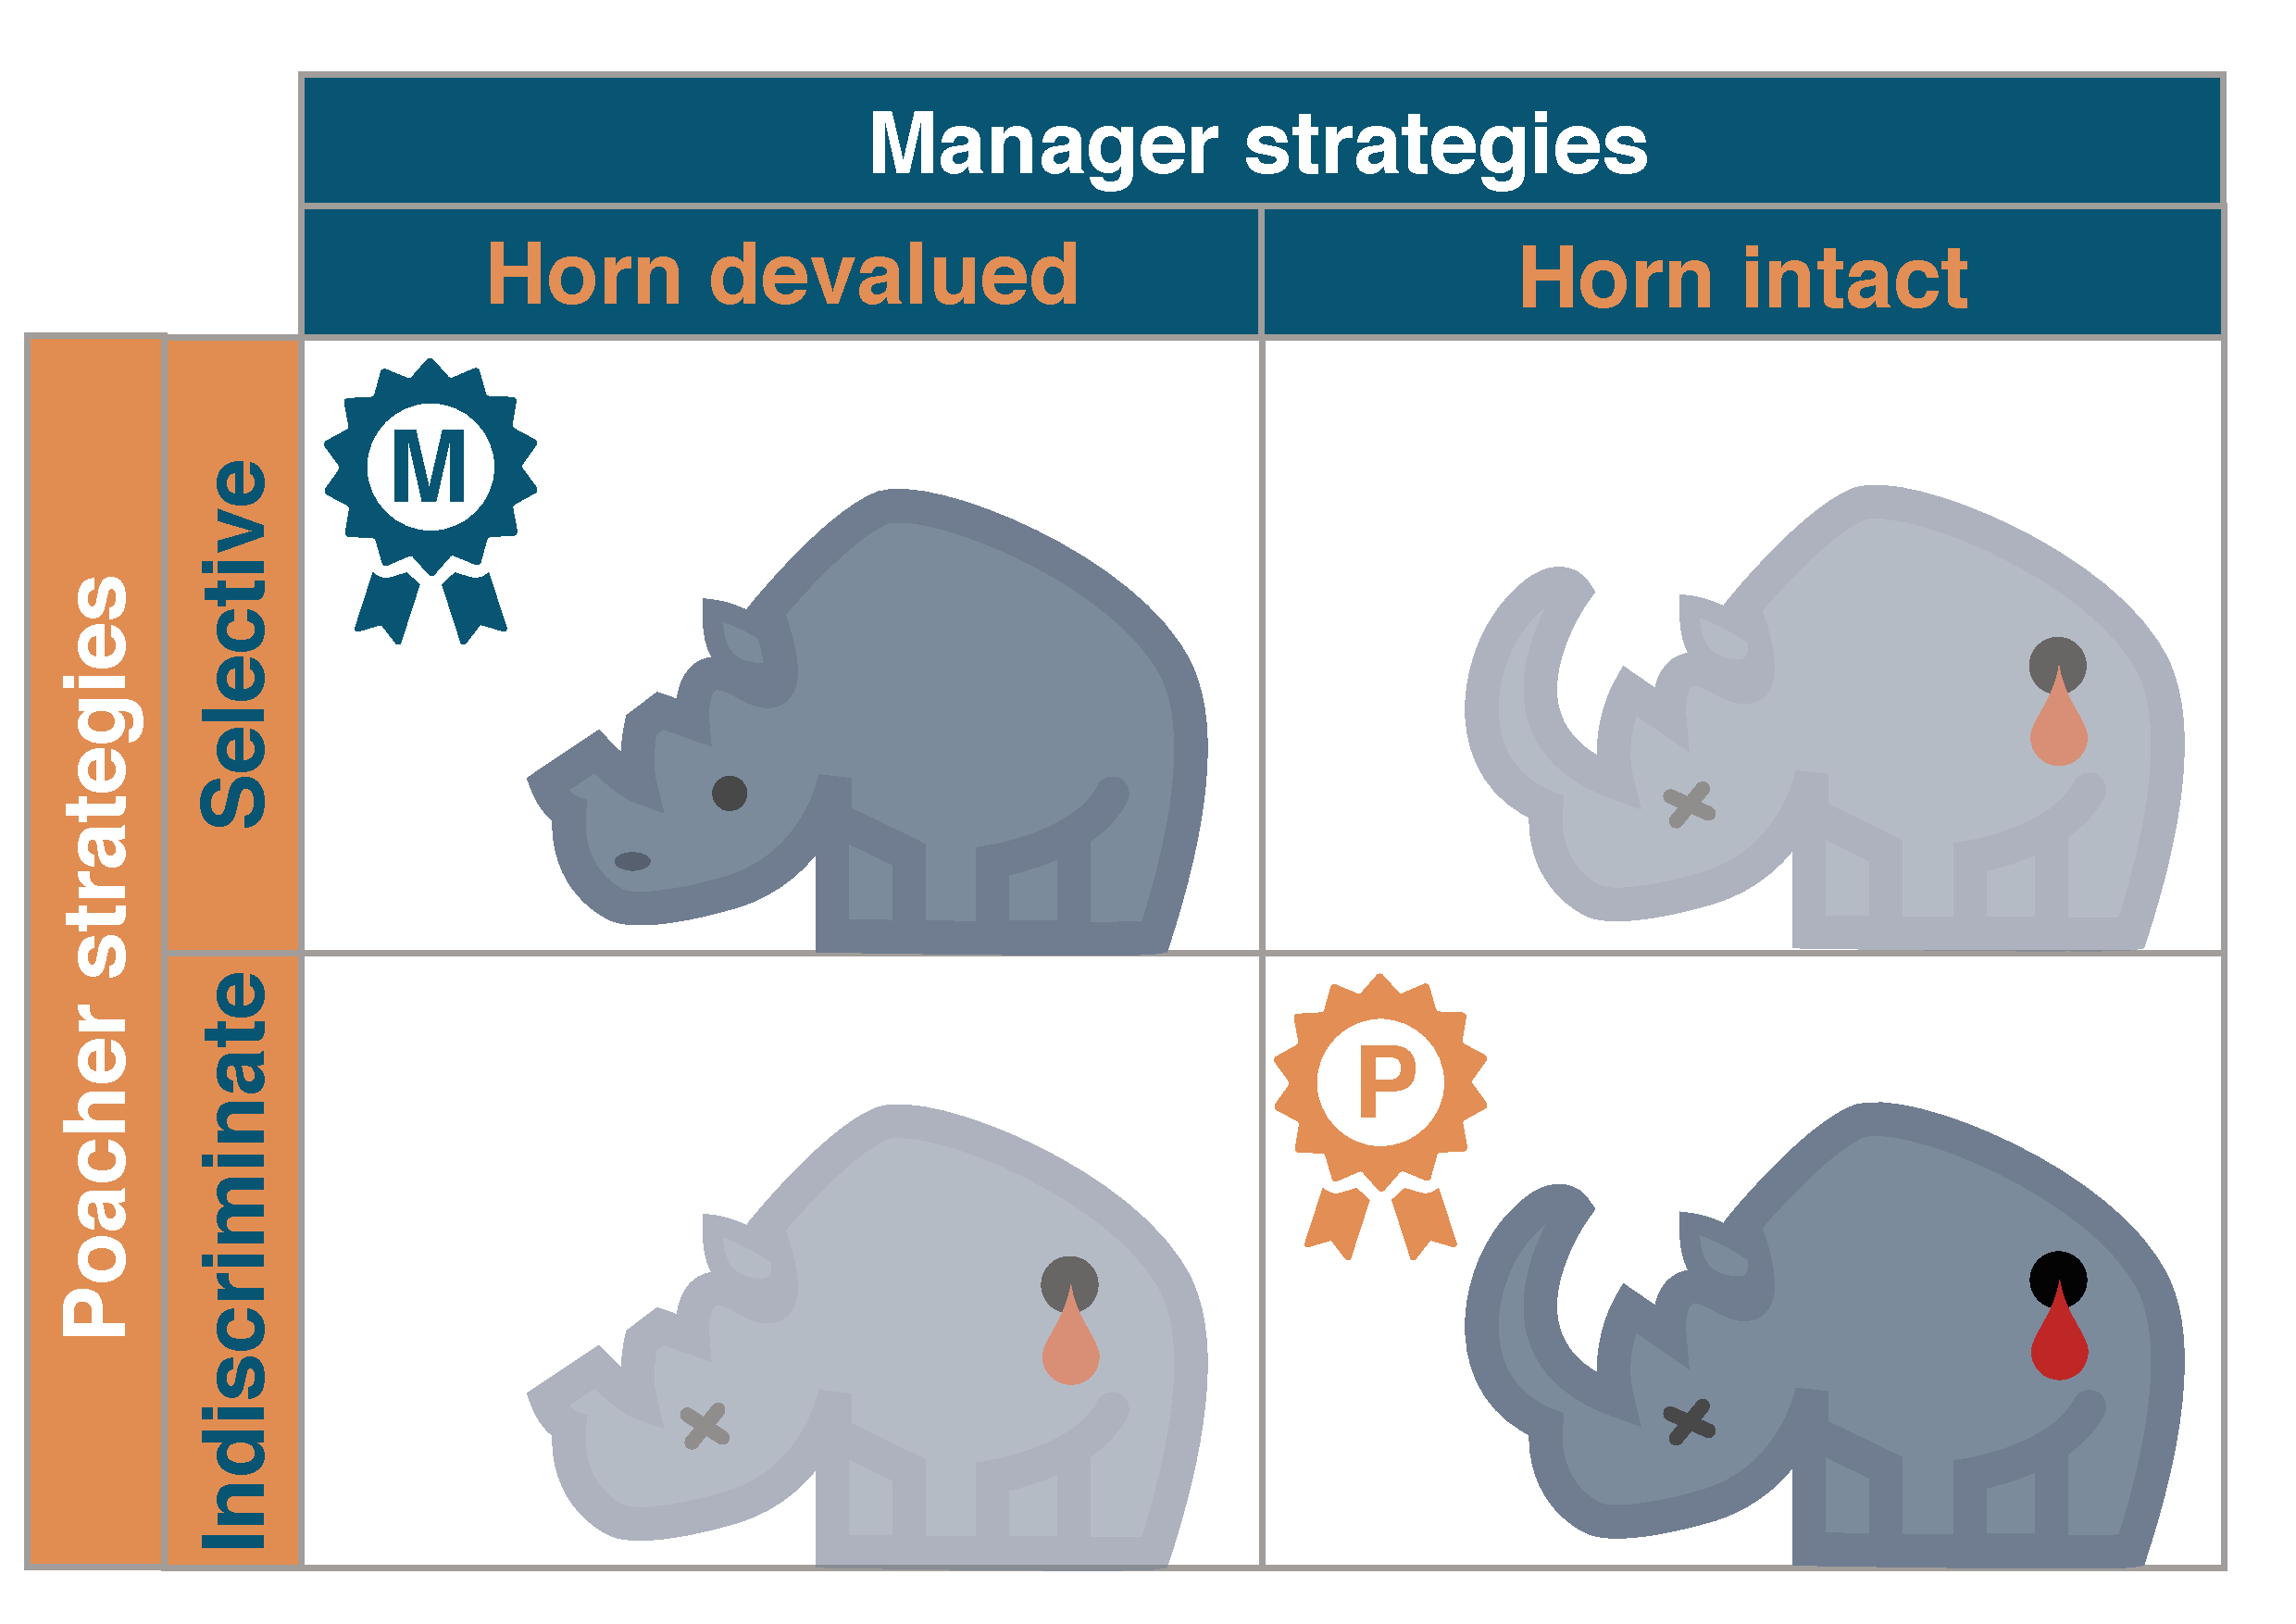
\includegraphics[width=0.24\textwidth, height=0.25\textwidth]{static/RhinoPic.pdf}\hspace{10pt}
    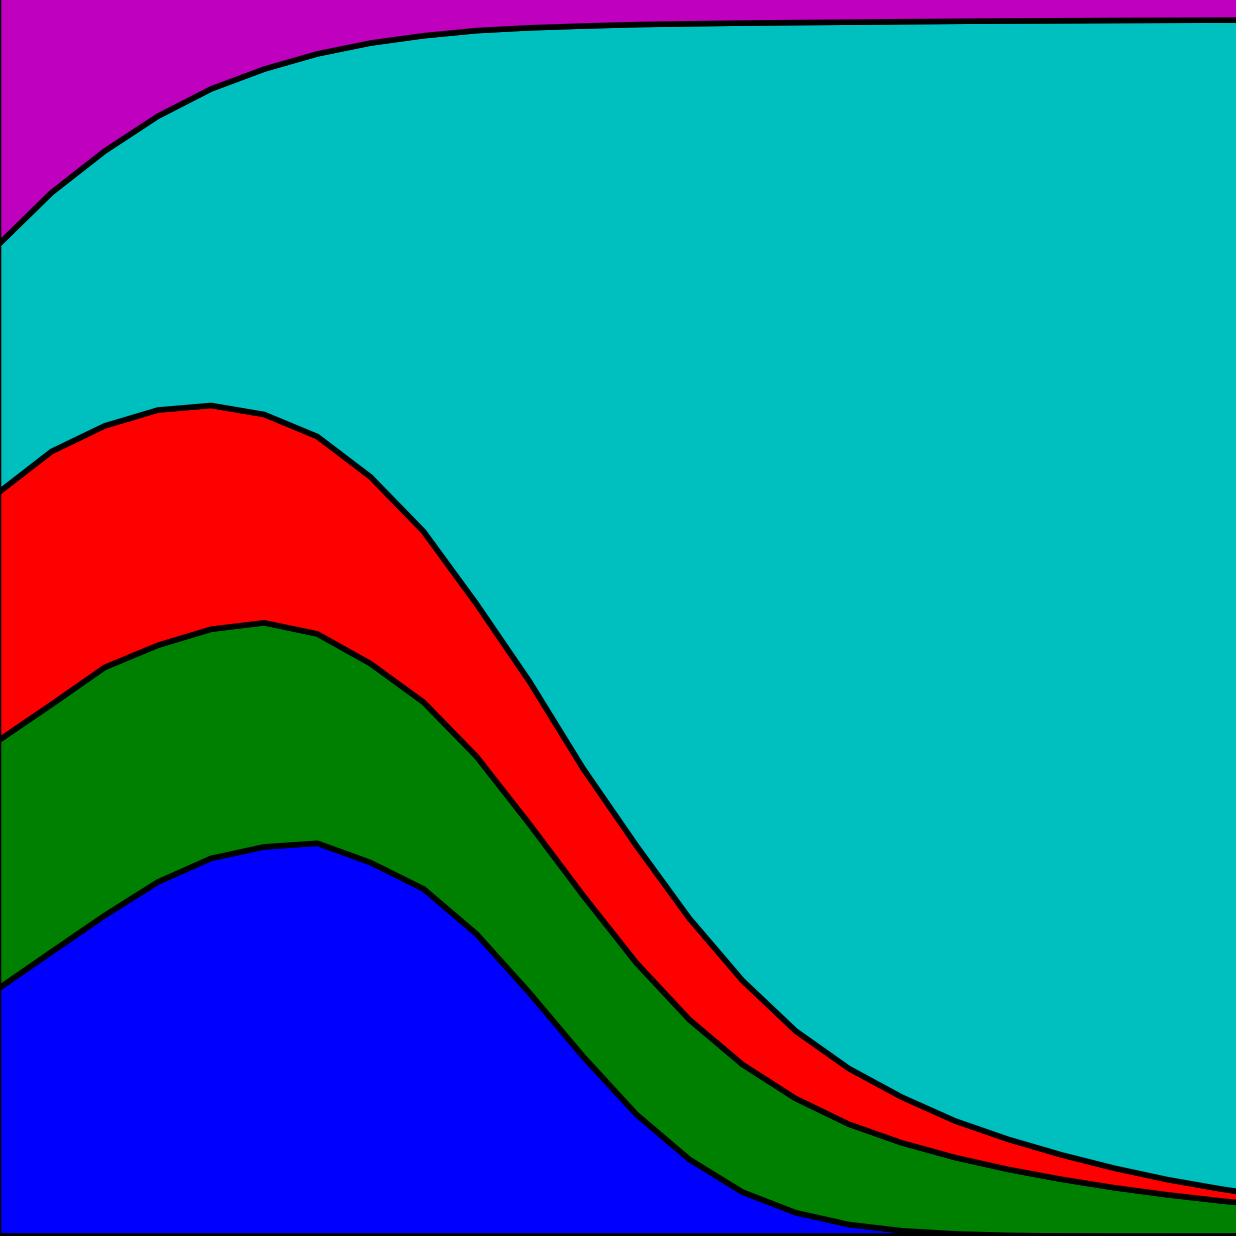
\includegraphics[width=0.24\textwidth]{static/axelrod-logo.png}\vspace{10pt}
    \end{center}
\end{frame}

\begin{frame}
	\begin{center}
\begin{todolist}
  \item[\done] Coursera Machine Learning.
  \item[\done] MA3604 Game Theory.
  \item[\done] NATCOR Stochastic Modeling.
\end{todolist}
    \end{center}
\end{frame}

\begin{frame}
\centering
\Huge Evolutionary Game Theory
\vfill
\large MA3604 Game Theory
\end{frame}

\begin{frame}
\centering
\includestandalone[width=0.8\textwidth]{static/evolutionary_stable}
\end{frame}

\begin{frame}
\centering
\includestandalone[width=0.4\textwidth]{static/stable_one}
\end{frame}

\begin{frame}
\centering
\includestandalone[width=0.4\textwidth]{static/stable_two}
\end{frame}

\begin{frame}
\centering
\includestandalone[width=0.4\textwidth]{static/stable_three}
\end{frame}

\begin{frame}
\centering
\includestandalone[width=0.9\textwidth]{static/evolutionary_steps}
\end{frame}


\begin{frame}
\begin{equation}
\begin{aligned}
u(\sigma, \chi) & = s u(S,\chi) +(1-s) u(\bar{S},\chi), \\
\end{aligned}
\end{equation}
\vspace{1cm}
\pause
\begin{equation}
\begin{aligned}
u(S,\chi) &= \theta(r,1) H \theta(r,x)^{-\alpha}
- \phi(r,1) (1-r)^{-\beta}
- \psi(r,1) F\psi(r, x)^{-\gamma} ,
\end{aligned}
\end{equation}
\vspace{0.3cm}
\pause
\begin{equation}
\begin{aligned}
u(\bar{S},\chi) &=  \theta(r,0) H \theta(r,x)^{-\alpha}
- \phi(r,0) (1-r)^{-\beta}
- \psi(r,0) F\psi(r, x)^{-\gamma}
\end{aligned}
\end{equation}
\end{frame}

\begin{frame}
\Large
\begin{equation*}
\begin{aligned}
\sigma_S & = (1,\ 0) \\
\sigma_{N} & = (0,\ 1) \\
\sigma_M & = (s^*,\ 1- s^*)
\end{aligned}
\end{equation*}
\end{frame}

\begin{frame}
\centering
\Huge Neural Networks
\vfill
\large Coursera Machine Learning
\end{frame}

\begin{frame}
\centering
\includestandalone[width=0.9\textwidth]{static/neural_nets}
\end{frame}

\begin{frame}
\centering
\includestandalone[width=0.9\textwidth]{static/neura_net_app}
\end{frame}


\begin{frame}
    \begin{center}
\begin{todolist}
  \item Summer School on Network Theory
  \item NATCOR Simulation.
  \item NATCOR Combinatorial Optimisation.
\end{todolist}
    \end{center}
\end{frame}

\begin{frame}
	\begin{center}
		\huge{\textbf{}}\\~\\
		\small{@NikoletaGlyn}\\
		\small{https://github.com/Nikoleta-v3}\\
	\end{center}
\end{frame}

\end{document}

